\documentclass{article}

\usepackage{minted}
\usepackage[most]{tcolorbox}
\usepackage{geometry}
\usepackage{enumitem}
\usepackage{hyperref}
\usepackage{hyperref}
\usepackage[parfill]{parskip}
\usepackage{wrapfig}
\usepackage{accsupp}

\geometry{margin=0.8in}
\definecolor{lightgreen}{rgb}{0.56, 0.93, 0.56}
\definecolor{moonstoneblue}{rgb}{0.45, 0.66, 0.76}
\definecolor{magenta}{rgb}{0.8,0.66,0.76}
\begin{document}
\begin{flushright}
Computational Biology ~\\
Tufts University Bio 35 ~\\
Fall 2021 ~\\ ~\\
\end{flushright}
\begin{center}{\textbf{\Large{Spotlight 8: Katie Pollard}}}\end{center}

\textit{Please note that in general I have taken/adapted the words of our Spotlight subjects from their own websites to describe their work. I have done this in an effort to maintain accuracy in describing their research programs. Please do not copy paste text from their papers/websites in your assignments!}

\begin{wrapfigure}{L}{0.15\textwidth}
\begin{center}
 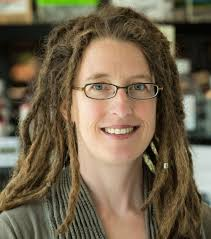
\includegraphics[width=0.16\textwidth]{images/katie-pollard.jpeg}
 \end{center}
\end{wrapfigure}
~\\ As part of our unit on functional genomics, we are going to explore the work of Prof. Katie Pollard. The Pollard lab develops statistical and computational methods to compare genomes and use the differences to decode how genomes work. Their analyses of massive sets of genomic and epigenomic data include investigating human genetic variation, understanding what makes humans unique compared to other species, and characterizing the genomic diversity of the human microbiome, the group of bacteria that populate our digestive system and other body sites. This evolutionary focus, coupled with rigorous statistical methods and bioinformatics tool development, gives the lab a unique perspective on human health and disease. Dr. Pollard is a faculty member at The Gladstone Institutes and UCSF.
~\\ 

Please watch the first 11.5 minutes of this video:
\begin{enumerate}
\item \texttt{\href{https://www.youtube.com/watch?v=4UtUZzQl-Xo}{https://www.youtube.com/watch?v=4UtUZzQl-Xo}}
\end{enumerate}
And read the following article about Prof. Pollard's work: 
\begin{enumerate}
\item \texttt{\href{https://www.nature.com/articles/nature05154.pdf}{https://www.nature.com/articles/nature05154.pdf}}
\end{enumerate}

\subsubsection*{Written Assignment} 
After reading about Katie Pollard please write a reflection (max one page) on what you discovered. You might wish to address some of the following: 

\begin{enumerate}
\item What was most interesting to you in reviewing these resources?
\item What did you learn from these resources about the fastest evolving regions of the human genome? How are computational tools employed in the detection of these regions?
\item What new questions do you have after reviewing these resources?
\item What do these resources tell you about the types of people that do computational biology, or their motivations?
\end{enumerate}

\EndAccSupp{}
\end{document}